% !TEX root = 0-main.tex
% !TEX encoding = UTF-8 Unicode
\chapter{Проектирование программного инструмента}
\label{cha:ch_2}


В качестве системы координат была выбрана классическая прямоугольная система, 
где одна координата обозначает номер строки в сетке, а вторая номер столбца.
у каждой ячейки максимум шесть соседних ячеек, это количество может уменьшаться 
из-за наличия закрытых ячеек.

\begin{figure}[h]
	\begin{center}
		\begin{minipage}[h]{0.47\linewidth}
			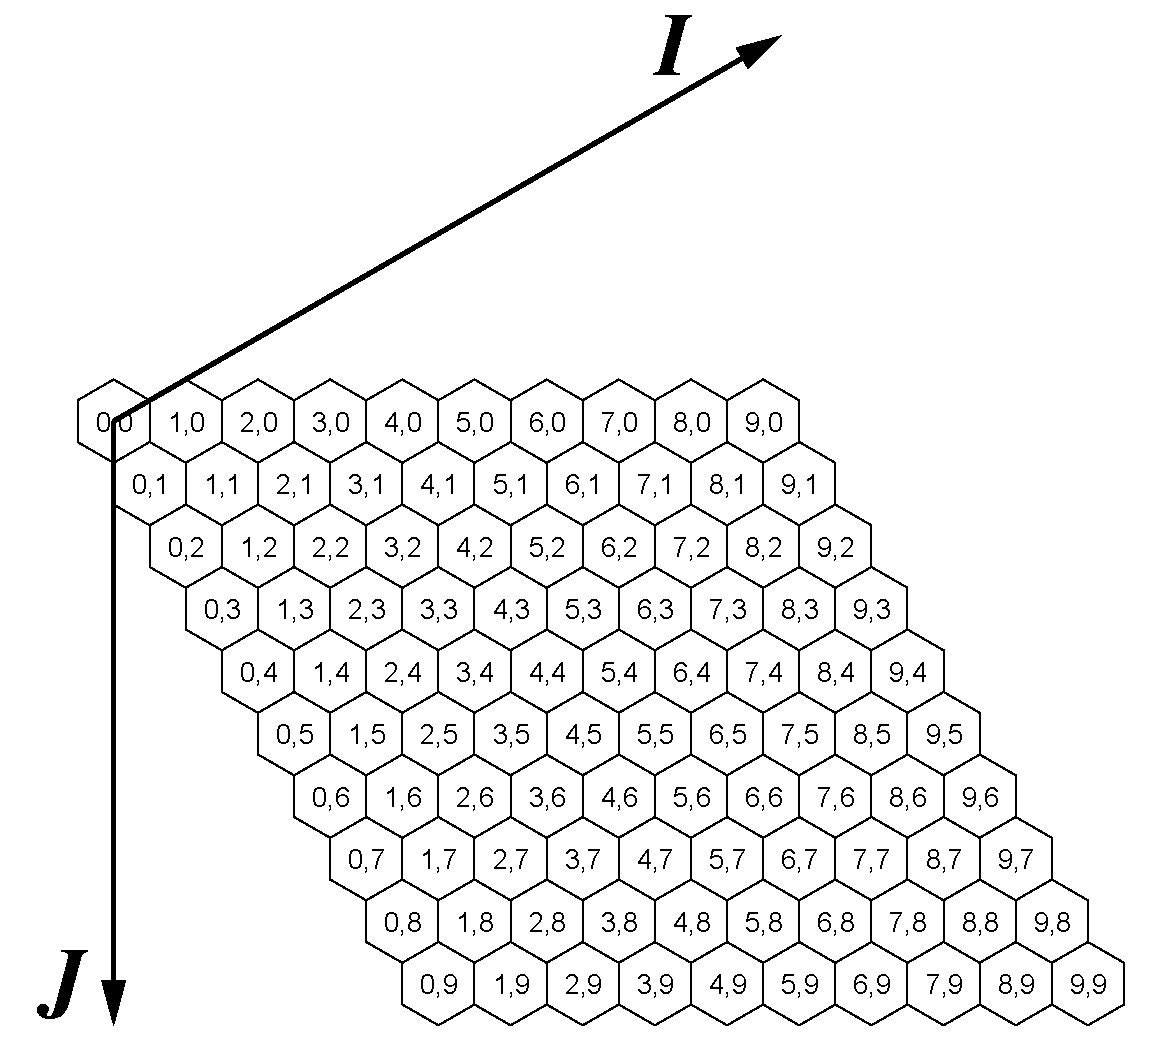
\includegraphics[width=1\linewidth]{inc/img/axies}
			\caption{Гексагональная сетка с ситемой координат.} %% подпись к рисунку
			\label{axis:cube} %% метка рисунка для ссылки на него
		\end{minipage}
		\hfill 
		\begin{minipage}[h]{0.47\linewidth}
			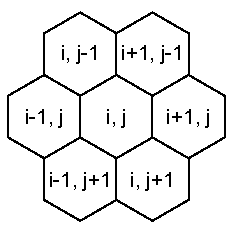
\includegraphics[width=1\linewidth]{inc/img/neibs}
			\caption{Соседние ячейки.}
			\label{axis:axial}
		\end{minipage}
	\end{center}
\end{figure}

\section{Описание классов и методов}
\begin{enumerate}
\item Класс \textbf{OffsetPoint}:
	\begin{enumerate}
	\item координата X
	\item координата Y
	\item перегрузка оператора проверки на равенство(==)
	\item перегрузка оператора проверки на неравенство (!=)
	\item перегрузка оператора сравнения (<)
	\end {enumerate}
\item Класс \textbf{HexagonGrid} (основной):
	
	Поля класса:
	\begin {enumerate}
	\item \textbf{dimension} - размерность сетки
	\item \textbf{hexSize} - размер шестиугольника (расстояние от центра до вершины)
	\item \textbf{gridWidth} - ширина сетки
	\item \textbf{gridHeight} - высота сетки
	\item \textbf{hexW} - ширина шестиугольника
	\item \textbf{hexH} - высота шестиугольника
	\item \textbf{start} - точка старта (типа OffsetPoint)
	\item \textbf{finish} - точка финиша (типа OffsetPoint)
	\item \textbf{fronts} - карта фронтов
	\item \textbf{path} - множество ячеек, входящих в путь
	\item \textbf{terminates} - множество закрытых ячеек
	\item \textbf{neighbours} - множество соседних ячеек к данной (public)
	\end {enumerate}
	Методы класса:
	\begin {enumerate}
	\item конструктор \textbf{HexagonGrid(int dimension, OffsetPoint start, OffsetPoint finish)}
	\item \textbf{drawSVG(string fileName)} - отрисовка сетки с учетом закрытых ячеек и пути
	\item \textbf{neighbours(int i, int j)} - алгоритм поиска соседних ячеек к данной 
	Осуществляет проверку всех вершин вокруг данной, и если они
	открыты, а также не выходят за пределы сетки, то добавляет в список. Возвращает список открытых
	соседних ячеек.
	\item \textbf{liAlg()} - реализация алгоритма Ли (пускает волну до нахождения финиша)
	Перебирает все ячеки, пока не найдет финишную или список открытых соседних ячеек не окажется пуст (в этом случае
	путь не найден, программа выходит из цикла).
	Каждая из этих ячеек в случае, если уже не входит в другой фронт волны, помечается номером на единицу 
	больше фронта данной ячейки. В итоге имеем карту, где каждому номеру фронта соответствует множество ячеек.
	
	\item \textbf{findPath()} - нахождение пути (двигается от финиша по фронтам волны)
	Начиная с финишной ячейки, ищет первую соседнюю с фронтом на единицу меньше и 
	добавляет ее в путь, пока не дойдет до ячейки старта.
	\item \textbf{BuildTerminates()} - построение закрытых ячеек случайным образом (private) 
	\end {enumerate}
\end {enumerate}
	



